
\guideline[g:nontext:figure_colorvisiondeficiency]
    {Figures: Ensure colors are distinguishable.}

\goodbadexample[{\cite[Fig.~3]{Wetzlinger2023HSCC}}]{
    % This file was created by matlab2tikz.
%
%The latest updates can be retrieved from
%  http://www.mathworks.com/matlabcentral/fileexchange/22022-matlab2tikz-matlab2tikz
%where you can also make suggestions and rate matlab2tikz.
%
\definecolor{mycolor1}{rgb}{0.00000,0.36078,0.67059}%
\definecolor{mycolor2}{rgb}{0.89020,0.10588,0.13725}%

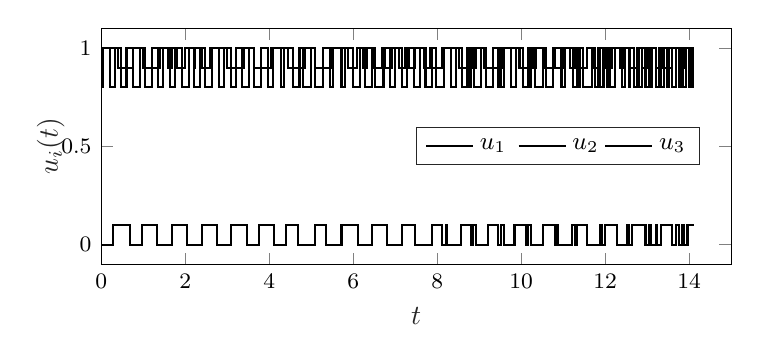
\begin{tikzpicture}

\begin{axis}[%
width=8cm,
height=3cm,
at={(0in,0in)},
scale only axis,
xmin=0.000,
xmax=15.000,
xlabel style={font=\color{white!15!black}},
xlabel={$t$},
ymin=-0.100,
ymax=1.100,
ylabel style={font=\color{white!15!black}, yshift=-8pt},
ylabel={$u_i(t)$},
axis background/.style={fill=white},
legend columns = 3,
legend style={legend cell align=left, font=\small, align=left, draw=white!15!black,
	at={(0.95,0.5)}, anchor=east,
	/tikz/column 2/.style={column sep=0.075cm}},
%legend image post style={line width = 1pt},
every tick label/.append style={font=\footnotesize}
]

\addplot [color=black, line width=0.75pt]
  table[row sep=crcr]{%
0.000	0.000\\
0.280	0.000\\
0.280	0.100\\
0.680	0.100\\
0.680	0.000\\
0.960	0.000\\
0.960	0.100\\
1.320	0.100\\
1.320	0.000\\
1.680	0.000\\
1.680	0.100\\
2.040	0.100\\
2.040	0.000\\
2.400	0.000\\
2.400	0.100\\
2.760	0.100\\
2.760	0.000\\
3.080	0.000\\
3.080	0.100\\
3.480	0.100\\
3.480	0.000\\
3.760	0.000\\
3.760	0.100\\
4.120	0.100\\
4.120	0.000\\
4.400	0.000\\
4.400	0.100\\
4.680	0.100\\
4.680	0.000\\
5.080	0.000\\
5.080	0.100\\
5.360	0.100\\
5.360	0.000\\
5.720	0.000\\
5.720	0.100\\
6.120	0.100\\
6.120	0.000\\
6.440	0.000\\
6.440	0.100\\
6.800	0.100\\
6.800	0.000\\
7.160	0.000\\
7.160	0.100\\
7.480	0.100\\
7.480	0.000\\
7.880	0.000\\
7.880	0.100\\
8.120	0.100\\
8.120	0.000\\
8.200	0.000\\
8.200	0.100\\
8.240	0.100\\
8.240	0.000\\
8.560	0.000\\
8.560	0.100\\
8.800	0.100\\
8.800	0.000\\
8.840	0.000\\
8.840	0.100\\
8.920	0.100\\
8.920	0.000\\
9.200	0.000\\
9.200	0.100\\
9.440	0.100\\
9.440	0.000\\
9.520	0.000\\
9.520	0.100\\
9.600	0.100\\
9.600	0.000\\
9.840	0.000\\
9.840	0.100\\
10.120	0.100\\
10.120	0.000\\
10.160	0.000\\
10.160	0.100\\
10.240	0.100\\
10.240	0.000\\
10.520	0.000\\
10.520	0.100\\
10.800	0.100\\
10.800	0.000\\
10.840	0.000\\
10.840	0.100\\
10.880	0.100\\
10.880	0.000\\
11.200	0.000\\
11.200	0.100\\
11.280	0.100\\
11.280	0.000\\
11.320	0.000\\
11.320	0.100\\
11.560	0.100\\
11.560	0.000\\
11.880	0.000\\
11.880	0.100\\
11.920	0.100\\
11.920	0.000\\
12.000	0.000\\
12.000	0.100\\
12.280	0.100\\
12.280	0.000\\
12.520	0.000\\
12.520	0.100\\
12.560	0.100\\
12.560	0.000\\
12.640	0.000\\
12.640	0.100\\
12.960	0.100\\
12.960	0.000\\
13.040	0.000\\
13.040	0.100\\
13.080	0.100\\
13.080	0.000\\
13.200	0.000\\
13.200	0.100\\
13.240	0.100\\
13.240	0.000\\
13.320	0.000\\
13.320	0.100\\
13.600	0.100\\
13.600	0.000\\
13.680	0.000\\
13.680	0.100\\
13.760	0.100\\
13.760	0.000\\
13.840	0.000\\
13.840	0.100\\
13.880	0.100\\
13.880	0.000\\
13.960	0.000\\
13.960	0.100\\
14.120	0.100\\
};
\addlegendentry{$u_1$}

\addplot [color=black, line width=0.75pt]
  table[row sep=crcr]{%
0.000	0.800\\
0.040	0.800\\
0.040	1.000\\
0.200	1.000\\
0.200	0.800\\
0.320	0.800\\
0.320	1.000\\
0.480	1.000\\
0.480	0.800\\
0.600	0.800\\
0.600	1.000\\
0.760	1.000\\
0.760	0.800\\
0.920	0.800\\
0.920	1.000\\
1.040	1.000\\
1.040	0.800\\
1.200	0.800\\
1.200	1.000\\
1.360	1.000\\
1.360	0.800\\
1.480	0.800\\
1.480	1.000\\
1.640	1.000\\
1.640	0.800\\
1.760	0.800\\
1.760	1.000\\
1.920	1.000\\
1.920	0.800\\
2.080	0.800\\
2.080	1.000\\
2.200	1.000\\
2.200	0.800\\
2.360	0.800\\
2.360	1.000\\
2.480	1.000\\
2.480	0.800\\
2.640	0.800\\
2.640	1.000\\
2.800	1.000\\
2.800	0.800\\
2.920	0.800\\
2.920	1.000\\
3.080	1.000\\
3.080	0.800\\
3.200	0.800\\
3.200	1.000\\
3.360	1.000\\
3.360	0.800\\
3.520	0.800\\
3.520	1.000\\
3.640	1.000\\
3.640	0.800\\
3.800	0.800\\
3.800	1.000\\
3.960	1.000\\
3.960	0.800\\
4.080	0.800\\
4.080	1.000\\
4.280	1.000\\
4.280	0.800\\
4.360	0.800\\
4.360	1.000\\
4.560	1.000\\
4.560	0.800\\
4.720	0.800\\
4.720	1.000\\
4.800	1.000\\
4.800	0.800\\
5.000	0.800\\
5.000	1.000\\
5.080	1.000\\
5.080	0.800\\
5.280	0.800\\
5.280	1.000\\
5.440	1.000\\
5.440	0.800\\
5.520	0.800\\
5.520	1.000\\
5.720	1.000\\
5.720	0.800\\
5.800	0.800\\
5.800	1.000\\
6.000	1.000\\
6.000	0.800\\
6.160	0.800\\
6.160	1.000\\
6.280	1.000\\
6.280	0.800\\
6.440	0.800\\
6.440	1.000\\
6.520	1.000\\
6.520	0.800\\
6.720	0.800\\
6.720	1.000\\
6.880	1.000\\
6.880	0.800\\
7.000	0.800\\
7.000	1.000\\
7.160	1.000\\
7.160	0.800\\
7.280	0.800\\
7.280	1.000\\
7.440	1.000\\
7.440	0.800\\
7.600	0.800\\
7.600	1.000\\
7.720	1.000\\
7.720	0.800\\
7.880	0.800\\
7.880	1.000\\
7.960	1.000\\
7.960	0.800\\
8.160	0.800\\
8.160	1.000\\
8.320	1.000\\
8.320	0.800\\
8.440	0.800\\
8.440	1.000\\
8.600	1.000\\
8.600	0.800\\
8.720	0.800\\
8.720	1.000\\
8.760	1.000\\
8.760	0.800\\
8.800	0.800\\
8.800	1.000\\
8.880	1.000\\
8.880	0.800\\
9.040	0.800\\
9.040	1.000\\
9.160	1.000\\
9.160	0.800\\
9.320	0.800\\
9.320	1.000\\
9.440	1.000\\
9.440	0.800\\
9.480	0.800\\
9.480	1.000\\
9.520	1.000\\
9.520	0.800\\
9.600	0.800\\
9.600	1.000\\
9.760	1.000\\
9.760	0.800\\
9.880	0.800\\
9.880	1.000\\
10.040	1.000\\
10.040	0.800\\
10.160	0.800\\
10.160	1.000\\
10.200	1.000\\
10.200	0.800\\
10.240	0.800\\
10.240	1.000\\
10.320	1.000\\
10.320	0.800\\
10.520	0.800\\
10.520	1.000\\
10.600	1.000\\
10.600	0.800\\
10.760	0.800\\
10.760	1.000\\
10.960	1.000\\
10.960	0.800\\
11.040	0.800\\
11.040	1.000\\
11.240	1.000\\
11.240	0.800\\
11.320	0.800\\
11.320	1.000\\
11.360	1.000\\
11.360	0.800\\
11.400	0.800\\
11.400	1.000\\
11.480	1.000\\
11.480	0.800\\
11.680	0.800\\
11.680	1.000\\
11.760	1.000\\
11.760	0.800\\
11.840	0.800\\
11.840	1.000\\
11.880	1.000\\
11.880	0.800\\
11.960	0.800\\
11.960	1.000\\
12.040	1.000\\
12.040	0.800\\
12.080	0.800\\
12.080	1.000\\
12.120	1.000\\
12.120	0.800\\
12.240	0.800\\
12.240	1.000\\
12.400	1.000\\
12.400	0.800\\
12.480	0.800\\
12.480	1.000\\
12.560	1.000\\
12.560	0.800\\
12.600	0.800\\
12.600	1.000\\
12.680	1.000\\
12.680	0.800\\
12.760	0.800\\
12.760	1.000\\
12.800	1.000\\
12.800	0.800\\
12.880	0.800\\
12.880	1.000\\
12.960	1.000\\
12.960	0.800\\
13.040	0.800\\
13.040	1.000\\
13.080	1.000\\
13.080	0.800\\
13.120	0.800\\
13.120	1.000\\
13.200	1.000\\
13.200	0.800\\
13.280	0.800\\
13.280	1.000\\
13.320	1.000\\
13.320	0.800\\
13.400	0.800\\
13.400	1.000\\
13.480	1.000\\
13.480	0.800\\
13.520	0.800\\
13.520	1.000\\
13.600	1.000\\
13.600	0.800\\
13.680	0.800\\
13.680	1.000\\
13.760	1.000\\
13.760	0.800\\
13.800	0.800\\
13.800	1.000\\
13.840	1.000\\
13.840	0.800\\
13.920	0.800\\
13.920	1.000\\
14.000	1.000\\
14.000	0.800\\
14.040	0.800\\
14.040	1.000\\
14.080	1.000\\
14.080	0.800\\
14.120	0.800\\
};
\addlegendentry{$u_2$}

\addplot [color=black, line width=0.75pt]
  table[row sep=crcr]{%
0.000	1.000\\
0.400	1.000\\
0.400	0.900\\
0.760	0.900\\
0.760	1.000\\
1.000	1.000\\
1.000	0.900\\
1.400	0.900\\
1.400	1.000\\
1.600	1.000\\
1.600	0.900\\
1.680	0.900\\
1.680	1.000\\
1.800	1.000\\
1.800	0.900\\
2.000	0.900\\
2.000	1.000\\
2.200	1.000\\
2.200	0.900\\
2.240	0.900\\
2.240	1.000\\
2.400	1.000\\
2.400	0.900\\
2.600	0.900\\
2.600	1.000\\
3.000	1.000\\
3.000	0.900\\
3.400	0.900\\
3.400	1.000\\
3.640	1.000\\
3.640	0.900\\
4.040	0.900\\
4.040	1.000\\
4.440	1.000\\
4.440	0.900\\
4.840	0.900\\
4.840	1.000\\
5.080	1.000\\
5.080	0.900\\
5.480	0.900\\
5.480	1.000\\
5.880	1.000\\
5.880	0.900\\
6.080	0.900\\
6.080	1.000\\
6.240	1.000\\
6.240	0.900\\
6.320	0.900\\
6.320	1.000\\
6.480	1.000\\
6.480	0.900\\
6.680	0.900\\
6.680	1.000\\
6.760	1.000\\
6.760	0.900\\
6.920	0.900\\
6.920	1.000\\
7.080	1.000\\
7.080	0.900\\
7.240	0.900\\
7.240	1.000\\
7.320	1.000\\
7.320	0.900\\
7.480	0.900\\
7.480	1.000\\
7.680	1.000\\
7.680	0.900\\
7.840	0.900\\
7.840	1.000\\
7.880	1.000\\
7.880	0.900\\
8.120	0.900\\
8.120	1.000\\
8.520	1.000\\
8.520	0.900\\
8.760	0.900\\
8.760	1.000\\
8.840	1.000\\
8.840	0.900\\
8.920	0.900\\
8.920	1.000\\
9.120	1.000\\
9.120	0.900\\
9.560	0.900\\
9.560	1.000\\
9.960	1.000\\
9.960	0.900\\
10.160	0.900\\
10.160	1.000\\
10.280	1.000\\
10.280	0.900\\
10.360	0.900\\
10.360	1.000\\
10.560	1.000\\
10.560	0.900\\
10.760	0.900\\
10.760	1.000\\
10.800	1.000\\
10.800	0.900\\
11.000	0.900\\
11.000	1.000\\
11.160	1.000\\
11.160	0.900\\
11.280	0.900\\
11.280	1.000\\
11.400	1.000\\
11.400	0.900\\
11.560	0.900\\
11.560	1.000\\
11.720	1.000\\
11.720	0.900\\
11.880	0.900\\
11.880	1.000\\
12.000	1.000\\
12.000	0.900\\
12.160	0.900\\
12.160	1.000\\
12.360	1.000\\
12.360	0.900\\
12.440	0.900\\
12.440	1.000\\
12.600	1.000\\
12.600	0.900\\
12.800	0.900\\
12.800	1.000\\
12.880	1.000\\
12.880	0.900\\
13.000	0.900\\
13.000	1.000\\
13.200	1.000\\
13.200	0.900\\
13.360	0.900\\
13.360	1.000\\
13.400	1.000\\
13.400	0.900\\
13.600	0.900\\
13.600	1.000\\
13.840	1.000\\
13.840	0.900\\
13.880	0.900\\
13.880	1.000\\
14.000	1.000\\
14.000	0.900\\
14.120	0.900\\
};
\addlegendentry{$u_3$}

\end{axis}

\end{tikzpicture}
}{
    % This file was created by matlab2tikz.
%
%The latest updates can be retrieved from
%  http://www.mathworks.com/matlabcentral/fileexchange/22022-matlab2tikz-matlab2tikz
%where you can also make suggestions and rate matlab2tikz.
%
\definecolor{mycolor1}{rgb}{0.00000,0.36078,0.67059}%
\definecolor{mycolor2}{rgb}{0.89020,0.10588,0.13725}%

\tikzsetnextfilename{figure_cvd_good}
\begin{tikzpicture}

\begin{axis}[%
width=8cm,
height=3cm,
at={(0in,0in)},
scale only axis,
xmin=0.000,
xmax=15.000,
xlabel style={font=\color{white!15!black}},
xlabel={$t$},
ymin=-0.100,
ymax=1.100,
ylabel style={font=\color{white!15!black}, yshift=-8pt},
ylabel={$u_i(t)$},
axis background/.style={fill=white},
legend columns = 3,
legend style={legend cell align=left, font=\small, align=left, draw=white!15!black,
	at={(0.95,0.5)}, anchor=east,
	/tikz/column 2/.style={column sep=0.075cm}},
%legend image post style={line width = 1pt},
every tick label/.append style={font=\footnotesize}
]

\addplot [color=black, line width=0.75pt]
  table[row sep=crcr]{%
0.000	0.000\\
0.280	0.000\\
0.280	0.100\\
0.680	0.100\\
0.680	0.000\\
0.960	0.000\\
0.960	0.100\\
1.320	0.100\\
1.320	0.000\\
1.680	0.000\\
1.680	0.100\\
2.040	0.100\\
2.040	0.000\\
2.400	0.000\\
2.400	0.100\\
2.760	0.100\\
2.760	0.000\\
3.080	0.000\\
3.080	0.100\\
3.480	0.100\\
3.480	0.000\\
3.760	0.000\\
3.760	0.100\\
4.120	0.100\\
4.120	0.000\\
4.400	0.000\\
4.400	0.100\\
4.680	0.100\\
4.680	0.000\\
5.080	0.000\\
5.080	0.100\\
5.360	0.100\\
5.360	0.000\\
5.720	0.000\\
5.720	0.100\\
6.120	0.100\\
6.120	0.000\\
6.440	0.000\\
6.440	0.100\\
6.800	0.100\\
6.800	0.000\\
7.160	0.000\\
7.160	0.100\\
7.480	0.100\\
7.480	0.000\\
7.880	0.000\\
7.880	0.100\\
8.120	0.100\\
8.120	0.000\\
8.200	0.000\\
8.200	0.100\\
8.240	0.100\\
8.240	0.000\\
8.560	0.000\\
8.560	0.100\\
8.800	0.100\\
8.800	0.000\\
8.840	0.000\\
8.840	0.100\\
8.920	0.100\\
8.920	0.000\\
9.200	0.000\\
9.200	0.100\\
9.440	0.100\\
9.440	0.000\\
9.520	0.000\\
9.520	0.100\\
9.600	0.100\\
9.600	0.000\\
9.840	0.000\\
9.840	0.100\\
10.120	0.100\\
10.120	0.000\\
10.160	0.000\\
10.160	0.100\\
10.240	0.100\\
10.240	0.000\\
10.520	0.000\\
10.520	0.100\\
10.800	0.100\\
10.800	0.000\\
10.840	0.000\\
10.840	0.100\\
10.880	0.100\\
10.880	0.000\\
11.200	0.000\\
11.200	0.100\\
11.280	0.100\\
11.280	0.000\\
11.320	0.000\\
11.320	0.100\\
11.560	0.100\\
11.560	0.000\\
11.880	0.000\\
11.880	0.100\\
11.920	0.100\\
11.920	0.000\\
12.000	0.000\\
12.000	0.100\\
12.280	0.100\\
12.280	0.000\\
12.520	0.000\\
12.520	0.100\\
12.560	0.100\\
12.560	0.000\\
12.640	0.000\\
12.640	0.100\\
12.960	0.100\\
12.960	0.000\\
13.040	0.000\\
13.040	0.100\\
13.080	0.100\\
13.080	0.000\\
13.200	0.000\\
13.200	0.100\\
13.240	0.100\\
13.240	0.000\\
13.320	0.000\\
13.320	0.100\\
13.600	0.100\\
13.600	0.000\\
13.680	0.000\\
13.680	0.100\\
13.760	0.100\\
13.760	0.000\\
13.840	0.000\\
13.840	0.100\\
13.880	0.100\\
13.880	0.000\\
13.960	0.000\\
13.960	0.100\\
14.120	0.100\\
};
\addlegendentry{$u_1$}

\addplot [color=color_guideline, line width=0.75pt]
  table[row sep=crcr]{%
0.000	0.800\\
0.040	0.800\\
0.040	1.000\\
0.200	1.000\\
0.200	0.800\\
0.320	0.800\\
0.320	1.000\\
0.480	1.000\\
0.480	0.800\\
0.600	0.800\\
0.600	1.000\\
0.760	1.000\\
0.760	0.800\\
0.920	0.800\\
0.920	1.000\\
1.040	1.000\\
1.040	0.800\\
1.200	0.800\\
1.200	1.000\\
1.360	1.000\\
1.360	0.800\\
1.480	0.800\\
1.480	1.000\\
1.640	1.000\\
1.640	0.800\\
1.760	0.800\\
1.760	1.000\\
1.920	1.000\\
1.920	0.800\\
2.080	0.800\\
2.080	1.000\\
2.200	1.000\\
2.200	0.800\\
2.360	0.800\\
2.360	1.000\\
2.480	1.000\\
2.480	0.800\\
2.640	0.800\\
2.640	1.000\\
2.800	1.000\\
2.800	0.800\\
2.920	0.800\\
2.920	1.000\\
3.080	1.000\\
3.080	0.800\\
3.200	0.800\\
3.200	1.000\\
3.360	1.000\\
3.360	0.800\\
3.520	0.800\\
3.520	1.000\\
3.640	1.000\\
3.640	0.800\\
3.800	0.800\\
3.800	1.000\\
3.960	1.000\\
3.960	0.800\\
4.080	0.800\\
4.080	1.000\\
4.280	1.000\\
4.280	0.800\\
4.360	0.800\\
4.360	1.000\\
4.560	1.000\\
4.560	0.800\\
4.720	0.800\\
4.720	1.000\\
4.800	1.000\\
4.800	0.800\\
5.000	0.800\\
5.000	1.000\\
5.080	1.000\\
5.080	0.800\\
5.280	0.800\\
5.280	1.000\\
5.440	1.000\\
5.440	0.800\\
5.520	0.800\\
5.520	1.000\\
5.720	1.000\\
5.720	0.800\\
5.800	0.800\\
5.800	1.000\\
6.000	1.000\\
6.000	0.800\\
6.160	0.800\\
6.160	1.000\\
6.280	1.000\\
6.280	0.800\\
6.440	0.800\\
6.440	1.000\\
6.520	1.000\\
6.520	0.800\\
6.720	0.800\\
6.720	1.000\\
6.880	1.000\\
6.880	0.800\\
7.000	0.800\\
7.000	1.000\\
7.160	1.000\\
7.160	0.800\\
7.280	0.800\\
7.280	1.000\\
7.440	1.000\\
7.440	0.800\\
7.600	0.800\\
7.600	1.000\\
7.720	1.000\\
7.720	0.800\\
7.880	0.800\\
7.880	1.000\\
7.960	1.000\\
7.960	0.800\\
8.160	0.800\\
8.160	1.000\\
8.320	1.000\\
8.320	0.800\\
8.440	0.800\\
8.440	1.000\\
8.600	1.000\\
8.600	0.800\\
8.720	0.800\\
8.720	1.000\\
8.760	1.000\\
8.760	0.800\\
8.800	0.800\\
8.800	1.000\\
8.880	1.000\\
8.880	0.800\\
9.040	0.800\\
9.040	1.000\\
9.160	1.000\\
9.160	0.800\\
9.320	0.800\\
9.320	1.000\\
9.440	1.000\\
9.440	0.800\\
9.480	0.800\\
9.480	1.000\\
9.520	1.000\\
9.520	0.800\\
9.600	0.800\\
9.600	1.000\\
9.760	1.000\\
9.760	0.800\\
9.880	0.800\\
9.880	1.000\\
10.040	1.000\\
10.040	0.800\\
10.160	0.800\\
10.160	1.000\\
10.200	1.000\\
10.200	0.800\\
10.240	0.800\\
10.240	1.000\\
10.320	1.000\\
10.320	0.800\\
10.520	0.800\\
10.520	1.000\\
10.600	1.000\\
10.600	0.800\\
10.760	0.800\\
10.760	1.000\\
10.960	1.000\\
10.960	0.800\\
11.040	0.800\\
11.040	1.000\\
11.240	1.000\\
11.240	0.800\\
11.320	0.800\\
11.320	1.000\\
11.360	1.000\\
11.360	0.800\\
11.400	0.800\\
11.400	1.000\\
11.480	1.000\\
11.480	0.800\\
11.680	0.800\\
11.680	1.000\\
11.760	1.000\\
11.760	0.800\\
11.840	0.800\\
11.840	1.000\\
11.880	1.000\\
11.880	0.800\\
11.960	0.800\\
11.960	1.000\\
12.040	1.000\\
12.040	0.800\\
12.080	0.800\\
12.080	1.000\\
12.120	1.000\\
12.120	0.800\\
12.240	0.800\\
12.240	1.000\\
12.400	1.000\\
12.400	0.800\\
12.480	0.800\\
12.480	1.000\\
12.560	1.000\\
12.560	0.800\\
12.600	0.800\\
12.600	1.000\\
12.680	1.000\\
12.680	0.800\\
12.760	0.800\\
12.760	1.000\\
12.800	1.000\\
12.800	0.800\\
12.880	0.800\\
12.880	1.000\\
12.960	1.000\\
12.960	0.800\\
13.040	0.800\\
13.040	1.000\\
13.080	1.000\\
13.080	0.800\\
13.120	0.800\\
13.120	1.000\\
13.200	1.000\\
13.200	0.800\\
13.280	0.800\\
13.280	1.000\\
13.320	1.000\\
13.320	0.800\\
13.400	0.800\\
13.400	1.000\\
13.480	1.000\\
13.480	0.800\\
13.520	0.800\\
13.520	1.000\\
13.600	1.000\\
13.600	0.800\\
13.680	0.800\\
13.680	1.000\\
13.760	1.000\\
13.760	0.800\\
13.800	0.800\\
13.800	1.000\\
13.840	1.000\\
13.840	0.800\\
13.920	0.800\\
13.920	1.000\\
14.000	1.000\\
14.000	0.800\\
14.040	0.800\\
14.040	1.000\\
14.080	1.000\\
14.080	0.800\\
14.120	0.800\\
};
\addlegendentry{$u_2$}

\addplot [color=color_example_bad, line width=0.75pt]
  table[row sep=crcr]{%
0.000	1.000\\
0.400	1.000\\
0.400	0.900\\
0.760	0.900\\
0.760	1.000\\
1.000	1.000\\
1.000	0.900\\
1.400	0.900\\
1.400	1.000\\
1.600	1.000\\
1.600	0.900\\
1.680	0.900\\
1.680	1.000\\
1.800	1.000\\
1.800	0.900\\
2.000	0.900\\
2.000	1.000\\
2.200	1.000\\
2.200	0.900\\
2.240	0.900\\
2.240	1.000\\
2.400	1.000\\
2.400	0.900\\
2.600	0.900\\
2.600	1.000\\
3.000	1.000\\
3.000	0.900\\
3.400	0.900\\
3.400	1.000\\
3.640	1.000\\
3.640	0.900\\
4.040	0.900\\
4.040	1.000\\
4.440	1.000\\
4.440	0.900\\
4.840	0.900\\
4.840	1.000\\
5.080	1.000\\
5.080	0.900\\
5.480	0.900\\
5.480	1.000\\
5.880	1.000\\
5.880	0.900\\
6.080	0.900\\
6.080	1.000\\
6.240	1.000\\
6.240	0.900\\
6.320	0.900\\
6.320	1.000\\
6.480	1.000\\
6.480	0.900\\
6.680	0.900\\
6.680	1.000\\
6.760	1.000\\
6.760	0.900\\
6.920	0.900\\
6.920	1.000\\
7.080	1.000\\
7.080	0.900\\
7.240	0.900\\
7.240	1.000\\
7.320	1.000\\
7.320	0.900\\
7.480	0.900\\
7.480	1.000\\
7.680	1.000\\
7.680	0.900\\
7.840	0.900\\
7.840	1.000\\
7.880	1.000\\
7.880	0.900\\
8.120	0.900\\
8.120	1.000\\
8.520	1.000\\
8.520	0.900\\
8.760	0.900\\
8.760	1.000\\
8.840	1.000\\
8.840	0.900\\
8.920	0.900\\
8.920	1.000\\
9.120	1.000\\
9.120	0.900\\
9.560	0.900\\
9.560	1.000\\
9.960	1.000\\
9.960	0.900\\
10.160	0.900\\
10.160	1.000\\
10.280	1.000\\
10.280	0.900\\
10.360	0.900\\
10.360	1.000\\
10.560	1.000\\
10.560	0.900\\
10.760	0.900\\
10.760	1.000\\
10.800	1.000\\
10.800	0.900\\
11.000	0.900\\
11.000	1.000\\
11.160	1.000\\
11.160	0.900\\
11.280	0.900\\
11.280	1.000\\
11.400	1.000\\
11.400	0.900\\
11.560	0.900\\
11.560	1.000\\
11.720	1.000\\
11.720	0.900\\
11.880	0.900\\
11.880	1.000\\
12.000	1.000\\
12.000	0.900\\
12.160	0.900\\
12.160	1.000\\
12.360	1.000\\
12.360	0.900\\
12.440	0.900\\
12.440	1.000\\
12.600	1.000\\
12.600	0.900\\
12.800	0.900\\
12.800	1.000\\
12.880	1.000\\
12.880	0.900\\
13.000	0.900\\
13.000	1.000\\
13.200	1.000\\
13.200	0.900\\
13.360	0.900\\
13.360	1.000\\
13.400	1.000\\
13.400	0.900\\
13.600	0.900\\
13.600	1.000\\
13.840	1.000\\
13.840	0.900\\
13.880	0.900\\
13.880	1.000\\
14.000	1.000\\
14.000	0.900\\
14.120	0.900\\
};
\addlegendentry{$u_3$}

\end{axis}

\end{tikzpicture}
}

\noindent
Color vision deficiency affects approximately $8\%$ of men and $0.5\%$ of women worldwide, or roughly $1$ in $12$ men and $1$ in $200$ women \footfullcite{Gordon1998}.
As a result, it is highly likely that some readers would benefit from color choices that accommodate this condition.
The ``bad'' version in the example above uses only black lines to simulate how indistinguishable colors can appear to individuals with color vision deficiency.
